\section{Hybrid pixels}
   Hybrid pixels are made of two parts (fig. \ref{fig:hybrid_DEPFET_scheme}a), the sensor and the electronics: for each pixel these two parts are welded together through microconnection (bump bond).\\  
   Hybrid pixels provide a practical system where readout and sensor, being independent, can be optimized separately, although the sensors cannot be tested without being connected to the readout and this represents a significant pratical issue.\\
   In addition the particular and sophisticated procedure to bond sensor and ASIC (application specific integrated circuit) makes them difficult to produce, delicate, especially for high levels of radiation, and also expensive. \\
   A critical parameter for accelerator experiments is the material budget, which represents the main limit factor for momentum measurement resolution in a magnetic field; since hybrid pixels are thicker ($\sim$ hundreds of $\mu m$) than monolithic ones (even less than 100 $\mu m$), using the latter the material budget can be down by a third: typical value for hybrid pixels is 1.5 \% $X_0$ per layer, while for monolithic 0.5 \% $X_0$.\\
   Among other disadvantages of hybrid pixels there is the bigger power consumption that implies, by the way, a bigger cooling system leading in turn to an increase in material too.\\

   \begin{figure}
      \begin{subfigure}{.5\textwidth}
      \centering
      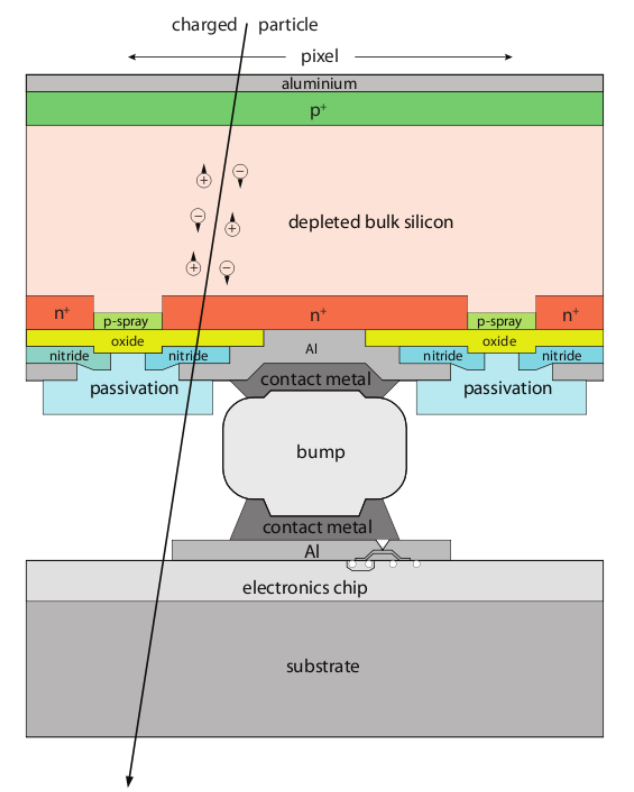
\includegraphics[width=.6\linewidth]{figures/Pixel_detectors/hybrid_scheme.png}
      \end{subfigure}%
      \begin{subfigure}{.5\textwidth}
      \centering
      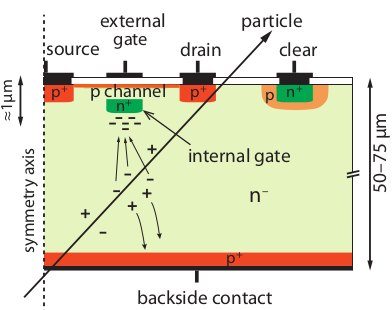
\includegraphics[width=.8\linewidth]{figures/Pixel_detectors/DEPFET_scheme.png}
      \end{subfigure}
      \caption{Concept cross section of hybrid pixel (a) and of a DEPFET (b)}
      \label{fig:hybrid_DEPFET_scheme}
   \end{figure} 

   DEPFET are the first attempt towards the integration of the front end (FE) on the sensor bulk: they are typically mounted on a hybrid structure but they also integrate the first amplification stage.\\
   Each pixel implements a MOSFET (metal-oxide-semiconductor field-effect transistor) transistor (a p-channel in fig. \ref{fig:hybrid_DEPFET_scheme}b): an hole current flows from source to drain which is controlled by the external gate and the interlan gate together. The intenal gate is made by a deep $n+$ implant towards which electrons drfit after being created in the deplation region (to know how the signal is created in a pixel detector look at appendix \ref{Appendix:pixels_overview}); the accumulation of electrons in the region underneath the n implant changes the gate potential and controls the transistor current.\\
   DEPFET typically have a good S/N ratio: this is principally due the amplification on-pixel and the large depletion region. But, since they need to be connect with ASIC the limiting factor still is the material budget.
   %hanno anche un capacità piccol

\section{CMOS MAPS and DMPAS}
   Monolitic active pixels accomodate on the same wafer both the sensor and the front end electronics, with the second one implanted on top. \\
   MAPS have been first proposed and realized in 1990s and their usage has been enabled by the development of the electronic sector which guarantees the decrease in CMOS transistors dimension at least every two years, as stated by the Moore's law\footnote{Moore's law states that logic density doubles every two years.}.\\
   As a matter of fact the dimension of componenents, their organization on the pixel area and logic density are important issues for the design and for the layout; typically different decisions are taken for different purposes.
   %Discorso fatto con Ludovico
   %sul fatto che i CMOSS tirano meno rispetto al circuito analogico.
   %Scrivi perchè si usano i CMOSS invece dei transistor: discorso sulla potenza e sull'elettronica digitale.\\      
   %UNA COSA (TROVATA SULLE SLIDES IFIP DI FORTI)È CHE ELETTRONICA RICHIEDE BASSA RESISTIVITÀ MENTRE ALTA RHO È RICHIESRA PER IL SENSORE. UN ALTRO PROBLEMA DEL CONNUBIO TRA LE DUE PARTI È LA TEMPERATURA: ELETTRONICA LAVORA ANCHE A T ALTE, SENSORE NO PERCHÈ SENNO HAI LEACKAGE CURRENT\\

   Monolithic active pixel can be distinguish beteween two main category: MAPS and depleted MAPS (DMAPS).\\
   \begin{figure}
      \centering
      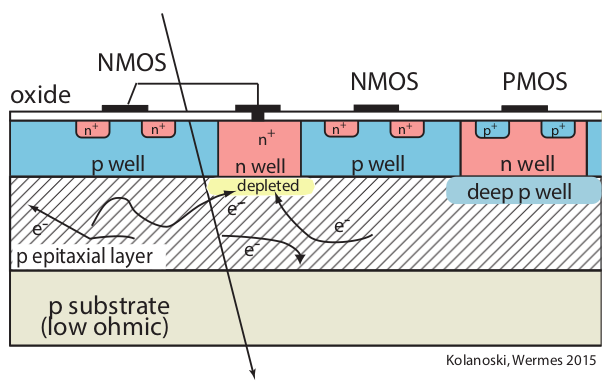
\includegraphics[width=.4\linewidth]{figures/Pixel_detectors/MAPS_scheme.png}
      \caption{Concept cross section of CMOS MPAS pixel}
      \label{fig:MAPS_scheme}
   \end{figure}
   MAPS (figure a \ref{fig:MAPS_scheme}) have typically an epitaxyal layer in range 1-20 $\mu m$ and because they are not depleted, the charge is mainly collected by diffusion rather then by drift. This makes the path of charges created in the bulk longer than usual, therefore they are slow (of order of 100 ns) and the collection could be partial expecially after the irradiation of the detector (look at \ref{Appendix:pixels_overview} for radiation damages), when the trapping probability become highter. \\
   In figure \ref{fig:MAPS_scheme} is shown as example of CMOS MAPS: the sensor in the scheme implements an n well as collection diode; to avoid the others n wells (which contain PMOS transistor) of the electronic circuit would compete in charge collection and to shield the CMOS circuit from the substrate, additionaly underlying deep p well are needed.
   DMAPS are instead MAPS depleated with $d$ typically in $\sim$ 25-150 $\mu m$ (eq. \ref{eq:deplation_d}) which extends from the diode to the deep p-well, and sometimes also to the the backside (in this case if one wants to collect the signal also on this electrode, additional process must be done).

   \subsection{DMAPS: large and small fill factor}
      There are two different sensor-design approaches (figure \ref{fig:large_small_sensor_scheme})
      to DMAPS:
      \begin{itemize}
         \item large fill factor: a large collection electrode that is a large deep n-well
      and that host the embedded electronics
         \item small fill factor: a small n-well is used as charge collection node
      \end{itemize}
      \begin{figure}
         \centering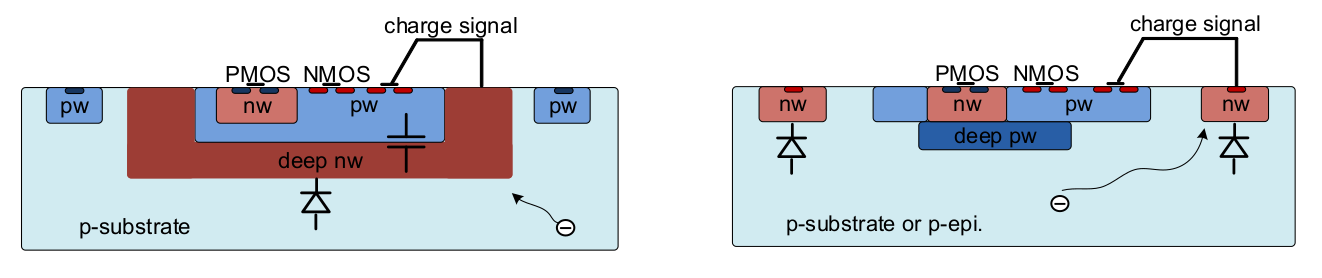
\includegraphics[width=12cm]{figures/Pixel_detectors/large_small_sensor_scheme.png}
         \caption{Concept cross section with large and small fill factor}
         \label{fig:large_small_sensor_scheme}
      \end{figure}
      To implement a uniform and stronger electric field, DMAPS often uses large electrode design that requires multiple wells (typically four including deep n and p wells); this layout adds on to the standard terms of the total capacity of the sensor a new term (fig. \ref{fig:DMAPS_capacity}), that contributes to the total amplifier input capacity. In addition to the capacity between pixels ($C_{pp}$) and between the pixel and the backside ($C_{b}$), a non negligible contribution comes from the capacities between wells ($C_{SW}$ and $C_{WW}$) needed to shield the embedded electronics. These capacities affect the thermal and 1/f noise of the charge amplifier and the $ \tau_{CSA}$ too:
      \begin{multicols}{2}
         \begin{equation}
            ENC^2 _ {thermal} \propto \frac{4}{3}\frac{kT}{g_m}\frac{C_D ^2}{\tau_{sh}}
         \end{equation}\quad 
         \begin{equation}
            \tau_{CSA} \propto \frac{1}{g_m}\frac{C_D}{C_f}
         \end{equation}
      \end{multicols} 
      where $g_m$ is the transconductance, $\tau_{sh}$ is the shaping time. \\
      Among the disadvantages coming from this large input capacity could be the coupling between the sensor and the electronics resulting in cross talk: noise induced by a signal on neighbouring electrodes; indeed, since digital switching in the FE electronics do a lot of oscillations, this problem is especially connected with the intra wells capacities.
      \begin{figure}[h!]
         \centering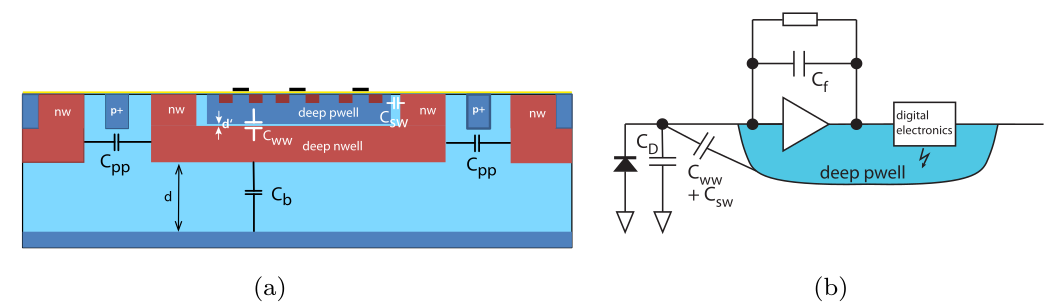
\includegraphics[width=12cm]{figures/Pixel_detectors/DMAPS_capacity.png}
         \caption{$C_{pp}$, $C_{b}$, $C_{WW}$, $C_{SW}$}
         \label{fig:DMAPS_capacity}
      \end{figure}
      So, larger charge collection electrode sensors provide a uniform electric field in the bulk that results in short drift path and so in good collection properties, especially after irradiation, when trapping probability can become an issue. The drawback of a large fill-factor is the large capacity ($\sim$100 fF): this contributes to the noise and to a speed penalty and to a larger possibility of cross talk.

      The small fill-factor variant, instead, benefits from a small capacity (5-20 fF), but suffers from a not uniform electric field and from all the issue related to that. \red{Ho già detto prima parlando dei MAPS, devo ripetere qui?}\\
      As we'll see these two different types of sensor require different amplifier: the large elctrode one is coupled with the charge sensitive amplifier, while the small one with voltage amplifier (sec \ref{subsec:preamplifier}).

      \begin{table}
         \begin{center}
         \begin{tabular}{|c | c |c |}
         \hline
         & small fill factor & large fill factor\\
         \hline
         \hline
         small sensor C & $\surd$ ($<$ 5 fF) & $\times$ ($\sim$ 100-200 fF)\\
         low noise & $\surd$ & $\times$\\
         low cross talk & $\surd$ & $\times$ \\
         velocity perfomances & $\surd$ & $\times$ ($\sim$ 100 ns)\\
         short drift paths & $\times$ & $\surd$ \\
         radiation hard & $\times$ & $\surd$ \\
         \hline
         \end{tabular}
         \caption{Small and large fill factor DMAPS characteristics}
         \label{tab:DMAPS_large_small_fillfactor}
         \end{center}
      \end{table}

   \subsection{A modified sensor}\ref{chap:a_modified_sensor}
      A process modification that has become the standard solution to combine the carateristic of a small fill factor sensor (small input amplifier capacity) and of large fill factor sensor (uniform electric field) is the one carried out for ALICE upgrade about ten years \cite{AProcessModification}.\\
      A compromise between the two sensors could also be making smaller pixels but this solution requires reducing the electronic circuit area, so a completelly new pixel layout should be think. The modification consists in inserting a low dose implant under the electrode and one its advantage lies in its versatility: both standard and modified sensor are often produced for testing in fact.

      Before the process modification the depletion region extends below the diode towards the substrate and it doesn't extend laterally so much even if a high bias is applied to the sensor (fig. \ref{fig:modified_process}). \\
      After, two distinct pn junctions are built: one between the deep p well and the $n^-$ layer, and the other between the $n^-$ and the $p^-$ epitaxial layer, extending to the all area of the sensor.\\ 
      Since deep p well and the p-substrate are separated by the deplation region, the two p electrodes can be biased separatelly\footnote{This is true in general, but it can be denied if other doping characteristics are implemented and we'll see that this is the case of TJ-Monopix1} and this is beneficial to enhance the vertical electric field component.\\
      The doping concentration is a trimmer parameter: it must be high enought to be greater than the epitaxial layer to prevent the punchthrought between p-well and the substrate, but it must also be lower enought to allow the depletion without reaching too high bias.
      \begin{figure}
         \centering
         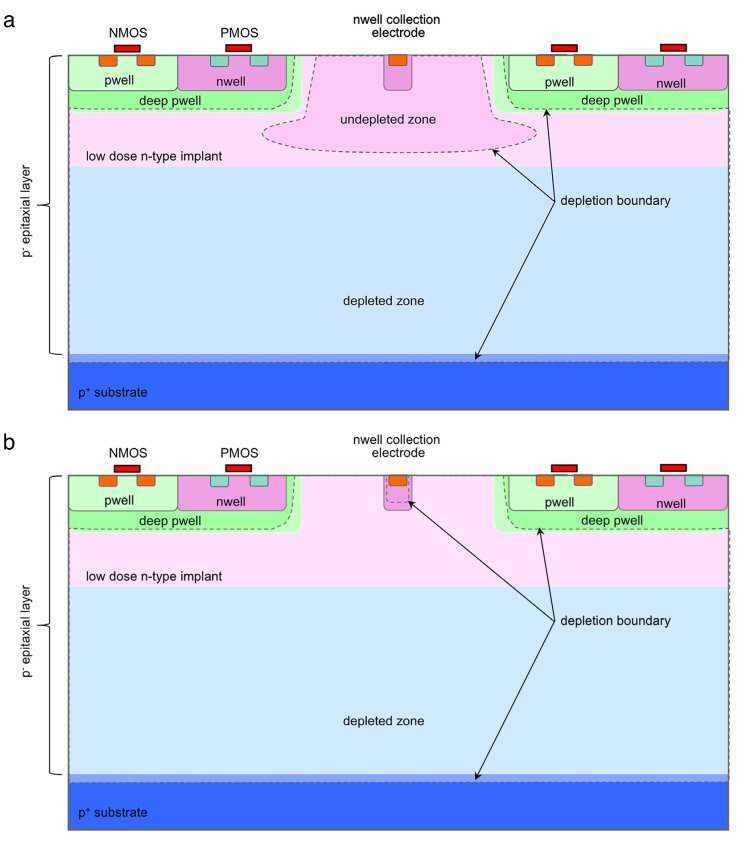
\includegraphics[width=.7\linewidth]{figures/Pixel_detectors/modified_process.png}
         \caption{A modified process for ALICE tracker detector: a low dose n implant is used to create a planar junction. In (a) the deplation is partial, while in (b) the pixel is fully depleted.}
         \label{fig:modified_process}
      \end{figure}

\section{Analog front end}
   After the creation of a signal on the electrode, the signal enters in the front end circuit (fig.\ref{fig:readout_scheme}), ready to be molded and transmitted out of chip.
   Low noise amplification, fast hit discrimination and an efficient, high-speed readout architecture, consuming as low power as possible  must be provided by the read out integrated electronics (ROIC).\\
   \begin{figure}
      \centering
      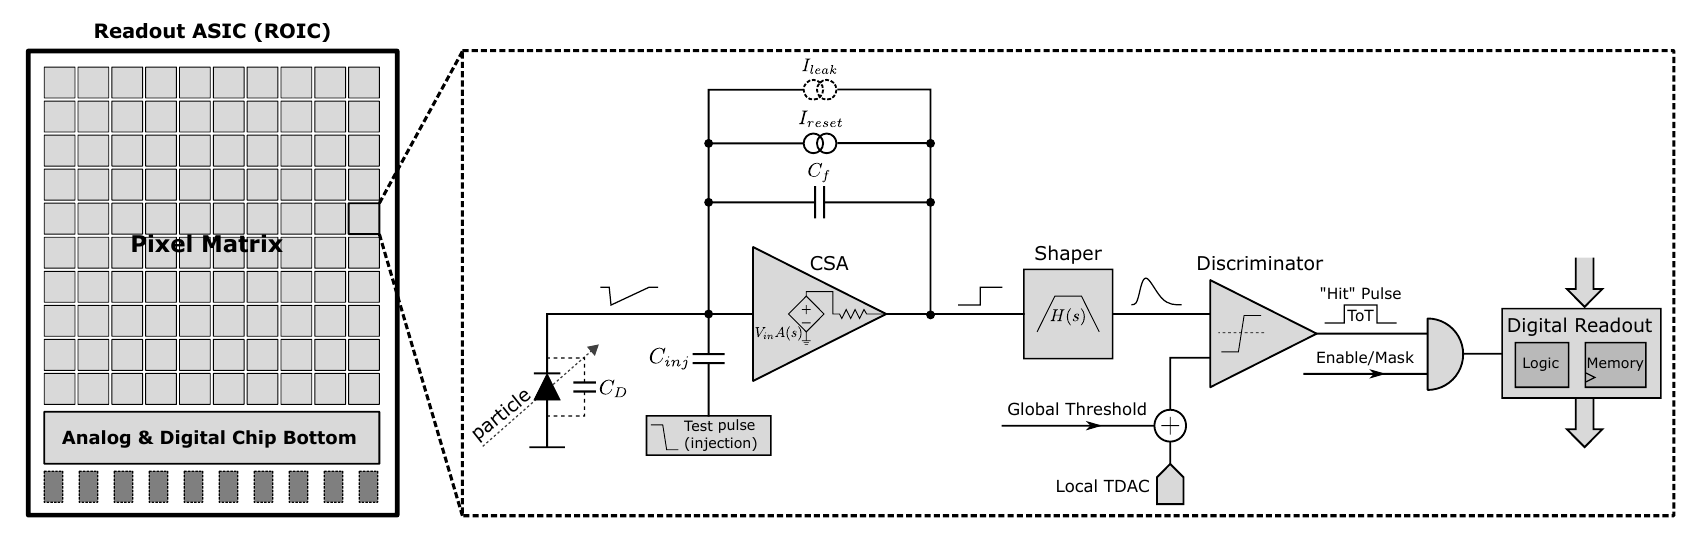
\includegraphics[width=1.\linewidth]{figures/Pixel_detectors/readout_scheme.png}
      \caption{Readout FE scheme: in this example the preamplifier is a charge sensitive one (CSA) but changing the capacitive feedback into a resistive one, this can be converted in a voltage or current amplifier.}
      \label{fig:readout_scheme}
   \end{figure}
   Let's take a look to the main steps of the analog front end chain: the preamplifier (that actually often is the only amplification stage) with a reset to the baseline mechanism and a leakage current compensation, a shaper (a band-pass filter) and finally a discriminator. The whole chain must be optimized and tuned to improve the S/N ratio: it is very important both not to have a large noise before the amplification stage in order to not moltiplicate that noise, and chose a reasonable threshold of the discriminator to cut noise-hits much as possible.

   \subsection{Preamplifier}\label{subsec:preamplifier}
      Even if circuits on the silicon crystal are only costruct by CMOS, a preamplifier can be modellized as an operational amplifier (OpAmp) where the gain is determined by the input and feedback impedance (first step in figure \ref{fig:readout_scheme}):
      \begin{equation}
         G = \frac{v_{out}}{v_{in}} = \frac{Z_{f}}{Z_{in}}
      \end{equation}
      Depending on whether a capacity or a resistance is used as feedback, respectevely a charge or a voltage amplifier is used: if the voltage input signal is large enought and have a sharp rise time, the voltage sensistive preamplifier is prefered. Consequently this flavor doesn't suit to large fill factor MAPS whose signal is already enought high: $v_{in} = Q/C_{D} \approx$ 3fC/100 pF = 0.03 mV, but it's fine for the small fill factor ones: $v_{in} = Q/C_{D} \approx$ 3fC/3 pF = 1 mV.

      In the case of a resistor feedback, if the signal duration time is longer than the discharge time ($\tau=R_S C_D$) of the detector the system works as current amplifier, as the signal is immediately trasmit to the amplifier; in the complementary case (signal duration longer than the discharge time) the system integrates the current on the $C_D$ and operates as a voltage amplifier.


   \subsection{ALPIDE-like front end}
      I've already mentioned ALICE pixel dector talking about the new process modification, now the ALICE name comes up again talking about FE: this is because ALPIDE (ALice PIxel DEtector) is one of the first MAPS detector (TowerJazz 180 nm CMOS) installed \footnote{It was installed in the Inner Tracking System during the second long shut down of the LHC in 2019}, therefore it is the current state of art and most of the following chips' FE are inspired by that, making it a standard in the FE design. \red{ARCADIA MD1 and TJ-Monopix1 are no exception, this is why I'm going to explain some principals characteristics of how it works}
      \begin{figure}[h!]
         \centering
         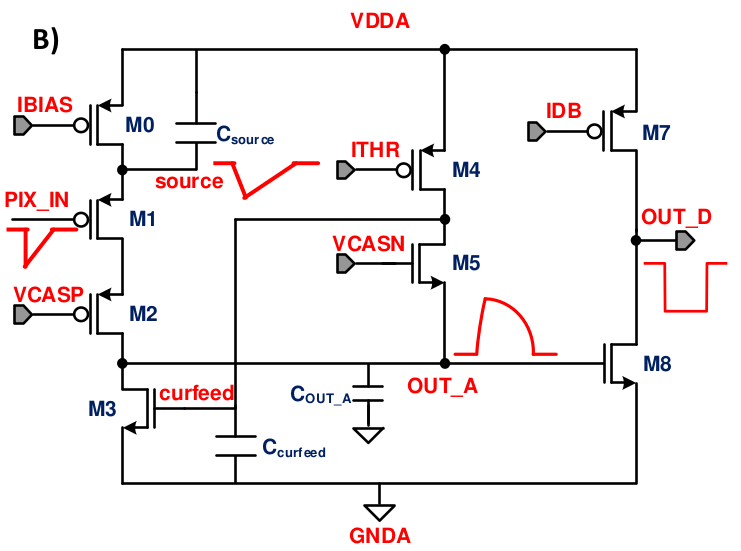
\includegraphics[width=.7\linewidth]{figures/Pixel_detectors/ALPIDE_FE.png}
         \caption{ALPIDE like FE}
         \label{fig:ALPIDE-like}
      \end{figure}

      The idea of the amplification stage is to transfer the charge from a bigger capacity\cite{ALPIDE-FE}, $C_{source}$, to a smaller one, $C_{out}$: the input transistor M1 with current source IBIAS acts as a source follower and this forces the source of M1 to be equal to the gate input  $\Delta V_{PIX\_IN} = Q_{IN}/C_{IN}$.
      \begin{equation}
         Q_{source} = C_{source} \Delta V_{PIX\_IN}
      \end{equation}
      The current in M2 and the charge accumulates on $C_{out}$ is fixed by the one on $C_{source}$:
      \begin{equation}
         \Delta V_{OUT\_A} = \frac{Q_{source}}{C_{OUT\_A}} = \frac{C_{source}\Delta V_{PIX\_IN}}{C_{OUT\_A}}  = \frac{C_{Source}}{C_{OUT\_A}}\frac{Q_{IN}}{C_{IN}}
      \end{equation}
      A second branch (M4, M5) is used to generate a low frequency feedback, where VCASN and ITHR set the baseline value of the signal on $C_{OUT\_A}$ and the velocity to goes down to the baseline.\\
      \red{IL RUOLO DI CURVFEED NON L'HO CAPITO, NELL'ARTICOLO C'È SCRITTO: The curfeed net, loaded with $C_{curfeed}$ capacitance and connected to the gate of M3 is adjusted for M3 to absorb IBIAS+ITHR.}\\
      Finally IDB defines the charge threshold with which the signal $OUT\_A$ must be compared: depending on if the signal is higher than the threshold or not, the $OUT\_D$ is high or low respectively.
      
\section{Readout logic}
   Readout logic includes the part of the circuit which takes the FE output singal, processes it and then trsamit it out of pixel and/or out of chip; depending on the situation of usage different readout characteristics must be provided. \\
   To store the analogical informations (i.e. charge collected, evolution of signal in time, ...) big buffers and a large bandwidth are needed; the problem that doesn't occur, or better occur only with really high rate, if one wants record only digital data (if one pixel is hit 1 is recorded, and if not 0 is recorded). 

   A common compromise often made is to save the time over threshold (ToT) of the pulse in clock cycle counts; this needs of relatively coarse requirement as ToT could be trimmer to be a dozen bits but, being correlated and hopefully being linear with the deposited charge by the impinging particle in the detector, it provides a sufficent information.
   The ToT digitalization usually takes advantage of the distribution of a clock (namely BCID,  bunch crossing identification) on the pixels matrix. The required timing precision is at least around 25 ns, that corresponds to the period of bunch collisions at LHC; for such reason a reasonable BCID-clock frequency for pixels detector is 40 MHz.\\
   Leading and trailing edges' timestamp of the pulse are saved on on pixel within a RAM unitl they have beeen read,  and then the ToT is obtained from their difference.
   \begin{figure}[h!]
      \centering
      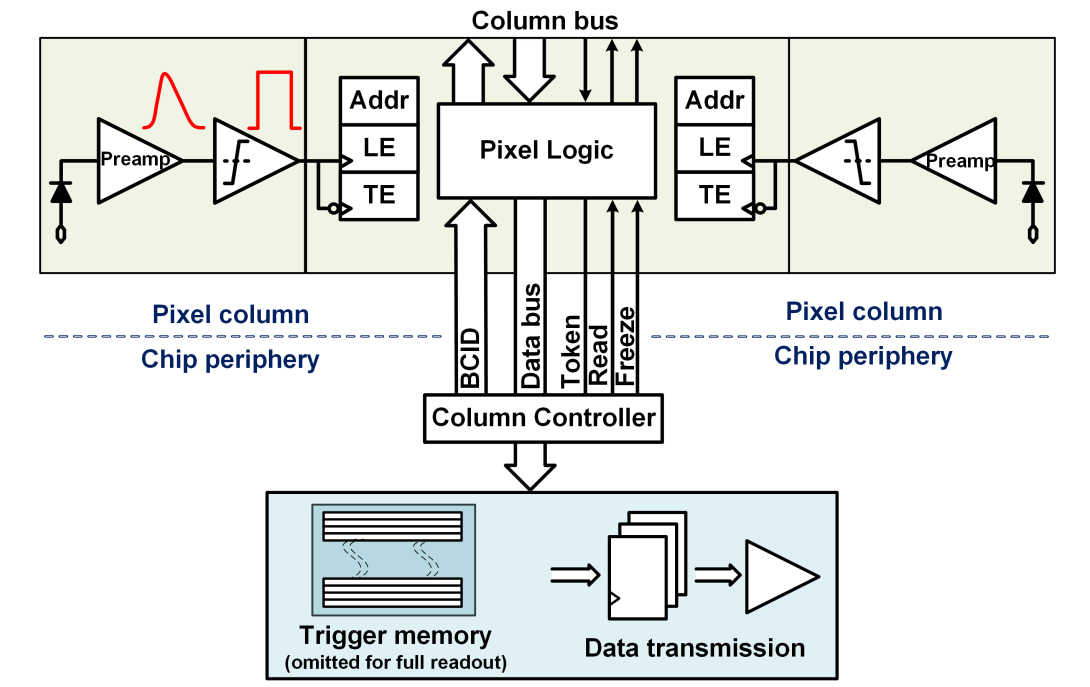
\includegraphics[width=.7\linewidth]{figures/Pixel_detectors/column_drain_RO.png}
      \caption{Column drain R/O scheme where ToT is saved}
      \label{fig:column_drain_RO-like}
   \end{figure}

   Moreover the readout architecture can be full, if every hit is read, or triggered, if a trigger system decides if the hit must be store or not. On one hand the triggered-readout needs buffers and storage memories, on the other the full readout, because there is no need to store hit data on chip, needs an high enough bandwidth.\\
   A triggered readout is foundamental in accelerator experiments where the quantity of data to store is too large to be hanled and some selection have to be applied by the trigger: to give an order of growth, at LHC more than 100 TBit/s of datas are produced but the storage data limit is about 100 MBit/s \cite{K-Wermes} (pag. 797).\\
   Typically the trigger signal is processed in a few $\mu s$ so the pixel gets it only after a hundred clock cycles from the hit arrival time: the buffer depht must than handle the higher trigger latency. 
 
   After having taken out the data from the pixel, it have to be transmitted to the end of column (EoC) where a serializer deliver it out of chip, typically to a FPGA.\\ 
   There are several ways of trasmitting data from pixel to the end of column: one of the most famous is the column-drain read out, developed for CMS and ATLAS experiments \cite{column-drain}. 
   All the pixels in a double-column share a data bus and only one pixel at a time, according to a priority chain, can be read. The reading order circuit is implemented by shift register (SR): when a hit arrives, the corresponding data, which can be made of timestamp and ToT, is temporarily stored on a RAM untill the SH does not allow the access to memory by data bus. \\
   Even if many readout architectures are based the column-drain one, it doesn't suit for large size matrices. The problem is that increasing the pixels on a column would also raise the number of pixels in the priority chain and that would results in a slowdown of the readout. 

   If there isn't any storage memory, the double-column behaves as a single server queue and the probability for a pixel of waiting a time $T$ greater than $t$, with an input hit rate on the column $\mu$ and an output bandwidt $B_W$ is \cite{Garcia-Review}:
   \begin{equation}
   P(T > t) = \frac{\mu}{B_W} e^{-( B_W-\mu )t}
   \label{eq:priority_chain_no_buffer}
   \end{equation}
   To avoid hit loss (let's neglect the contribution to the inefficency of the dead time $\tau$ due to the AFE), for example imponing $P(T > t)\sim\:$0.001, one obtains $(B_W -\mu)\:t_t\sim\:$6, where $t_t$ is the time needed to transfer the hit; since $t_t$ is small, one must have $B_W \gg \mu$, that means a high bandwidth \cite{Garcia-Review}.
   \begin{figure}[h!]
      \centering
      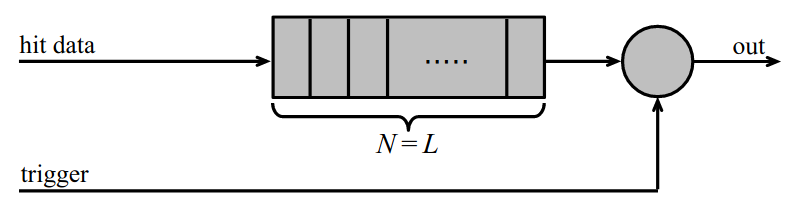
\includegraphics[width=.6\linewidth]{figures/Pixel_detectors/pipeline.png}
      \caption{Block diagram of a pipeline buffer: N is the dimension of memory buffer and L is the trigger latency expressed in BCID cycles}
      \label{fig:pipeline}
   \end{figure}

   Actually the previous one is an approximation since each pixel sees a different bandwidth depending on the position on the queue: the first one sees a full bandwidth, but the next sees a smaller one because occasionally it can be blocked by the previous pixel. Then the bandwidth seen by the pixel $i$ is $B_{i} = B - \sum _{j}\mu_{j}$, where $\mu_j$ is the hit rate of the $j$th pixel.\\
   The efficiency requirement on the bandwidth and the hit rate becomes: $B_{W,i} > \mu_{i}$, where the index $i$ means the constraint is for a single pixel; if all the N pixels on a column have the same rate $\mu = N\mu_{i}$, the condition reduces to $B_{W} > \mu$.
   The bandwidth must be chosen such that the mean time between hits of the last pixel in the readout chain is bigger than that.\\
   \red{In order to reduce the bandwidth a readout with zero suppression on pixel is typically employed; this means that only informations from channels where the signal exceeds the discriminator threshold are stored. QUalcosa sulla zero suprpession? La metto qui questa affermazione?}

   If instead there is a local storage until a trigger signal arrives, the input rate to column bus $\mu '$ is reduced compared to the hit rate $\mu$ as: $\mu'=\mu \times r \times t$, where $r$ is the trigger rate and $t$ is the bunch crossing period.
   In this situation there is a more relaxed constraint on the bandwidth, but the limiting factor is the buffer depht: the  amount of memory designed depends both on the expected rate $\mu$ and on the trigger latency $t$ as $\propto\mu \times t$, that means that the highter the trigger latency and the lower the hit rate to cope with. 

   In order to have an efficient usage of memory on pixels area it's convenient grouping pixels into regions with shared storage. Let's compare two different situations: in the first one a buffer is located on each pixel area, while in the second one a core of four pixels share a common buffer (this architecture is commonly called FE-I4). \\
   \begin{figure}[h!]
      \centering
      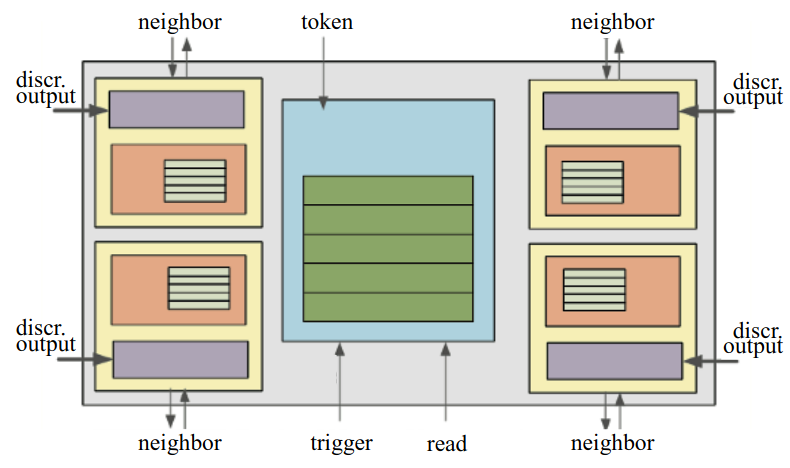
\includegraphics[width=.7\linewidth]{figures/Pixel_detectors/core.png}
      \caption{Block diagram of the FE-I4 PR organization. Read and memory
      management section is highlighted in light blue; latency counters and
      trigger management secrion are highlighted in green; hit processing blocks
      are highlighted in purple; ToT counters and ToT management units are
      highlighted in orange}
      \label{fig:core}
   \end{figure}
   Consider a 50 kHz single pixel hits rate and a trigger latency of 5 $\mu s$, the probability of lossing hits is: 
   \begin{equation}
      P(N > 1 | \nu) = 1-P(N = 0 | \nu) - P(N = 1 | \nu) = 1 - e^{-\nu} (1+\nu) \thickapprox 2.6 \% 
   \end{equation}    
   where I have assumed a Poissonian distribution with mean $\nu$ = 0.25 to describe the counts N.\\
   To get an efficiency $\epsilon$ greater than 99.9 \% a 3 hit depht buffer is needed: 
   \begin{equation}
      P(N > 3 | \nu) = 1-\sum_{i=0}^{3} P(N = i | \nu) < 0.1\%  
   \label{eq:efficiency_buffer}
   \end{equation} 
   Considering the second situation: if the average single pixel rate is still 50 kHz, grouping four pixels the mean number of hits per trigger latency is $\nu = 0.25 \times 4 = 1$. To get an efficiency of 99.9\% (eq. \ref{eq:efficiency_buffer}) a buffer depht of 5 hits in the four-pixels region, instead of 3 per pixels, is needed. 

